\chapter{Related Work}

% NOTE: compares, contrasts, synthesizes, and provides introspection about the available knowledge for
% a given topic or field

\section{CERTIFY} % (fold)
\label{sec:CERTIFY}
This thesis is carried out in conjunction with the CERTIFY project \cite{certifyproject2023}.
% TODO: (aver) explain goals of CERTIFY

The National Institute for Standard and Technology has a few ongoing projects and white papers on security related
mitigation methods for IoT devices.
% section CERTIFY (end)


\section{DLT-based Asset-Tracking} % (fold)
\label{sec:DLT-based Asset-Tracking}
\cite{neisse2017blockchain} analyzed how blockchain-based approaches might be used for data accountability and
provenance tracking under the then recently released GDPR legislation, highlighting challenges of scalability and
considering sharding as a method to address it. \cite{neisse2017blockchain} Further they also mentioned issues of
clonability of the tracked assets, which we can also correlate to the physical assets that are tracked inside
blockchain.
% section DLT-based Asset-Tracking (end)


\section{Cybersecurity of IoT Devices} % (fold)
\label{sec:Cybersecurity of IoT Devices}

In order to maintain participation rights for only valid users/clients, Manufacturer Usage Descriptions, MUDs, are
getting more and more relevant, as also the National Institute for Standards and Technology, NIST, have been considering
their use cases. \cite{dodson2021securing}

\subsection{SRAM-based PUF Readouts} % (fold)
\label{sub:SRAM-based PUF Readouts}
For this thesis we will not be implementing a sophisticated Designated Accrediting Authority, DAA, leading to the
assumption, that it will be implemented as part of another thesis. For our use-case we will refer to simple
hardcoded authentication, with a key being provided for each device by us and trusted by us for simplicity.

Nonetheless the topic is still relevant from a cybersecurity perspective and there have been a few attempts at creating
secure keys out of SRAM readouts, such as \cite{vinagrero2023sram} or \cite{Niya_Jeffrey_Stiller_2020}.
We will also be considering using SRAM-based PUF readouts in our device configurations in order to get DIDs that are
absolutely unique for each device.
% subsection SRAM-based PUF Readouts (end)

\subsection{Device Fingerprinting} % (fold)
\label{sub:Device Fingerprinting}
For classification of device capabilities NIST has been considering the usage of MUDs, so that devices do not step out
the bounds of their official and appointed capabilities. \cite{dodson2021securing}
% subsection Device Fingerprinting (end)

% section Cybersecurity of IoT Devices (end)

\section{Verified Credentials and Identity Management Technologies} % (fold)
\label{sub:Verified Credentials and Identity Management Technologies}

In the quest for the right technologies, we are only considering open source projects, so that we may extend frameworks
and applications with modules to fit out needs, which why there may be many options not listed in here.

\begin{table}
	\caption{Comparison of Identity Management and Verified Credentials related Software}
	\label{tab:Comparison of Identity Management and Verified Credentials related Software}
	\begin{center}
		\begin{tabular}[c]{|l|p{7cm}|l|}
			\hline
			\textbf{Technology Name}                  & Short Description                             & Main Feature \\
			\hline
			Hyperledger Aries \cite{hyperledger:wiki} & creating, transmitting and storing verifiable
			digital credentials                       & VC issuing                                                   \\
			\hline
			Hyperledger Indy \cite{hyperledger:wiki}  & Tools/Libraries for providing digital IDs
			rooted on Blockchains or DLTs             & DID and Tools                                                \\
			\hline
			IoTeX \cite{iotex-bc-platform}            & did                                           & did          \\
			\hline
		\end{tabular}
	\end{center}
\end{table}

\subsection{Decentralized Identity and Access Management for IoT (DIAM-IoT) Framework, 2020)} % (fold)
\label{sub:Decentralized Identity and Access Management for IoT}

\begin{figure}
	\begin{center}
		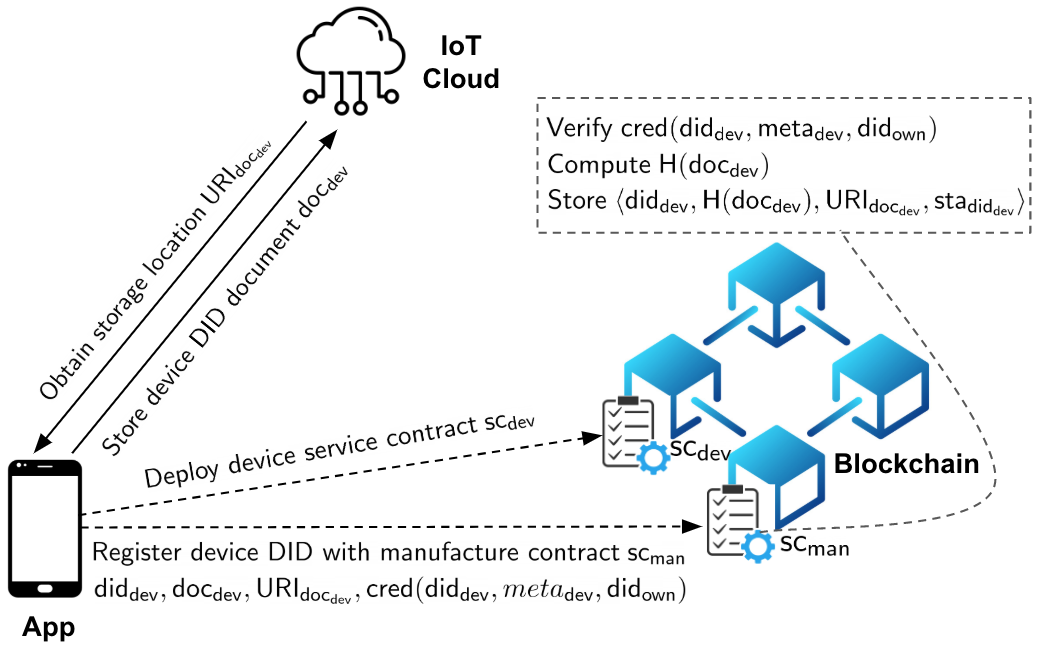
\includegraphics[width=0.95\textwidth]{figures/diam-iot-did-registration.png}
	\end{center}
	\caption{DIAM-IoT DID Registration Process \cite{diam-iot-2020}}
	\label{fig:diam-iot-did-registration}
\end{figure}

There has been a similar work in the field of our thesis, which has been made by \cite{diam-iot-2020}, who investigated
decentralized Identity and Access Management, IAM. They proposed a framework, DIAM-IoT, which incorporates DIDs and VCs
into the lifecycle of IoT devices, while building it up on blockchain as a bridge to connect IoT data silos.

They identified DID and global key-value databases as integral parts for building a self-sovereign identity system.

Their onboarding process includes the creation of a cryptocurrency wallet for manufacturers, through which each has to
stake some of the cryptocurrency tokens to deploy a smart contract for a new device. Those with poor products are
punished this way.

In contrast to our thesis, they refrained from using MUDs to specify device capabilities and designated each user with
their DID which is bound to a device that has a DID as well. Their use case is consumer oriented. Each user gets a
mobile application that can be used to do the device registration. A VC is generated by an IoT-Cloud after a successful
device binding (binding the user and a device). See Figure~\ref{fig:diam-iot-did-registration}.

Although they mention scalability in their paper, there is no hard data, to support one of our challenges, which is the
scalability and efficiency for using millions of devices.
% subsection Decentralized Identity and Access Management for IoT (end)

\subsection{Hyperledger Aries and Indy} % (fold)
\label{sec:Hyperledger Aries}

Hyperledger Aries is a graduated project from the Hyperledger foundation that focuses on on creating, transmitting and
storing verifiable digital credentials, with its infrastructure aimed at blockchain-rooted peer-2-peer interactions.

As mentioned in Section~\ref{sec:Verifiable Credentials and Identity Management}, Aries is already used to manage VCs
through compatible wallets in larger organizations such as the EU.
% subsection Hyperledger Aries (end)

\section{IoTeX} % (fold)
\label{sec:IoTeX}
IoTeX is a blockchain based framework focusing on decentralized application and IoT devices.
It provides functionalities such as blockchain, interconnections of decentralized applications, Dapps, using DIDs.
Architecturally is is quite similar to Ethereum, with a focus on IoT devices and also collaborating with Ethereum,
making it Ethereum Virtual Machine, EVM, compatible. Further DIDs are used to as on-chain identity framework that
enables users and devices to own their data, identity, and credentials. Further Real World Data Oracles convert real
world phenomena into verifiable and blockchain-ready data for use in the IoTeX Dapps.
IoTeX also supports Trusted Execution Environment, TEE, which is important for this thesis, i.e., for secure storage and
execution of certain applications and transactions.

Transactions are managed through the \textit{IOTX} token, e.g., to stake smart contracts as mentioned in
Section~\ref{sub:Decentralized Identity and Access Management for IoT}.

An advantage in using IoTeX would be, that it has already been used in IoT related projects, proving performance in the
area.

\begin{figure}
	\begin{center}
		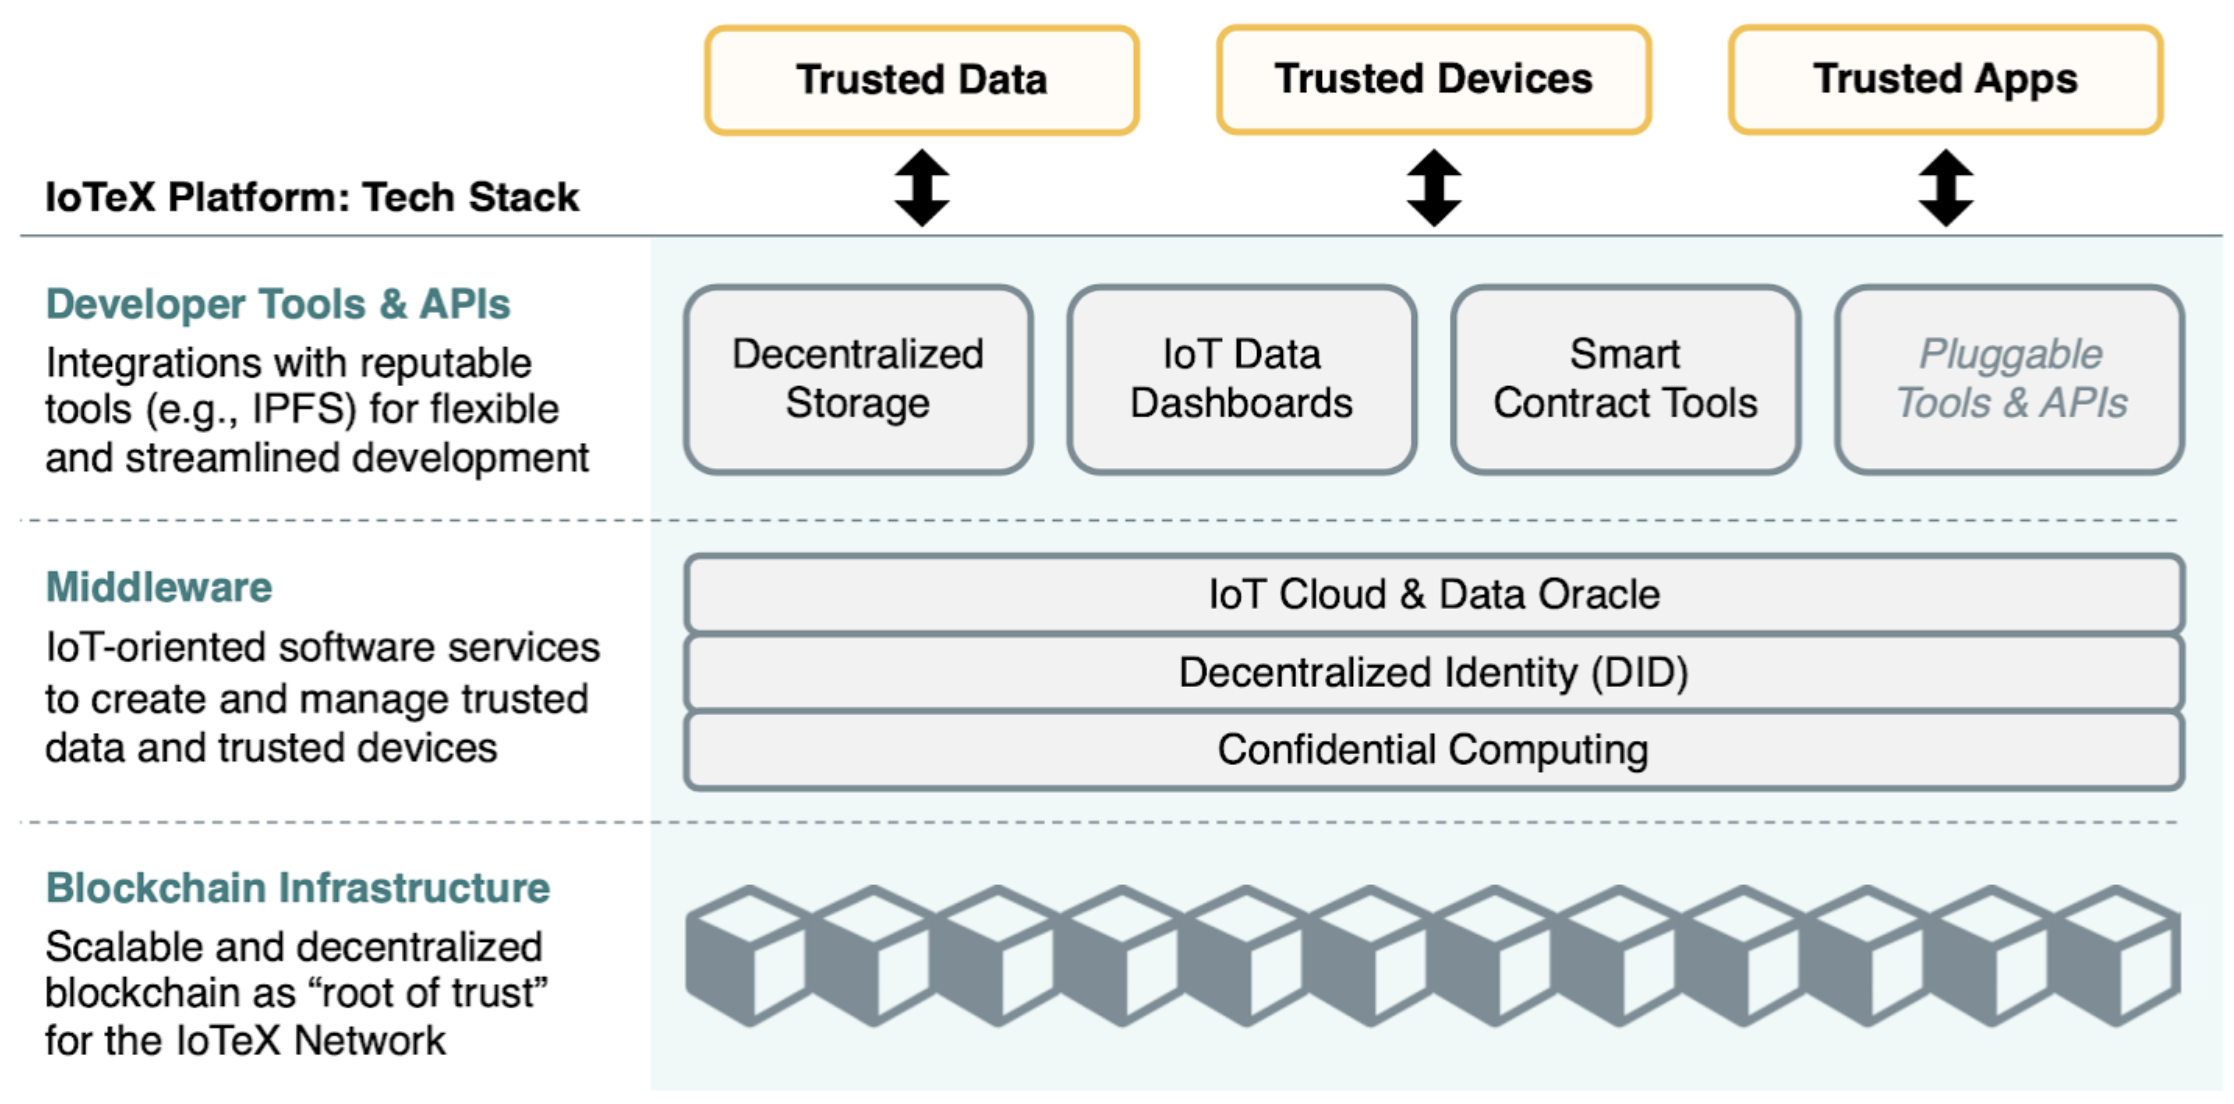
\includegraphics[width=0.95\textwidth]{figures/iotex-platform-stack.png}
	\end{center}
	\caption{IoTeX Platform Overview}
	\label{fig:iotex-platform-stack}
\end{figure}
% section IoTeX (end)

\section{Further non-DLT based IdM Frameworks} % (fold)
\label{sec:Further non-DLT based IdM Frameworks}
% https://identity.foundation/
% https://www.dock.io/post/decentralized-identity
% https://www.devicehive.com/#open+source
% https://docs.devicehive.com/docs

% section Further non-DLT based IdM Frameworks (end)

% section Verified Credentials and Identity Management Technologies (end)

\section{Blockchains} % (fold)
\label{sec:Blockchains}
\begin{table}
	\caption{Considered Blockchains}
	\label{tab:Considered Blockchains}
	\begin{center}
		\begin{tabular}[c]{|l|l|}
			\hline
			\textbf{Blockchain Name}                  & Key Characteristics  \\
			\hline
			Hyperledger Iroha \cite{hyperledger:wiki} & Permissioned Network \\
			\hline
			Ethereum                                  & Permissionless       \\
			\hline
			IoTeX \cite{iotex-bc-platform}            & Permissionless       \\
			\hline
		\end{tabular}
	\end{center}
\end{table}

\subsection{Ethereum} % (fold)
\label{sec:Ethereum}

Ethereum is a widely known and used blockchain.

Also there is the Hyperledger Besu \cite{hyperledger:wiki} client to interact with Ethereum.

There is the Ethereum Virtual Machine...
% subsection Ethereum (end)

\subsection{Hyperledger Iroha} % (fold)
\label{sub:Hyperledger Iroha}

Hyperledger Iroha is a relatively new and unknown blockchain from the Hyperledger Foundation \cite{hyperledger:wiki}.
% subsection Hyperledger Iroha (end)

\subsection{IoTeX (Blockchain)} % (fold)
\label{sec:IoTeX-Blockchain}
See Section~\ref{sec:IoTeX}.
% subsection IoTeX (Blockchain) (end)

% section Blockchains (end)

\section{Real-Time Operating Systems} % (fold)
\label{sec:Real-Time Operating Systems}

\subsection{TockOS} % (fold)
\label{sub:TockOS}

The CERTIFY project considers using TockOS for their implementation on the IoT devices.
Tock is a secure Real-Time Operating System, RTOS, designed to run on ARM and RISC-V based devices.

% subsection TockOS (end)
% section Real-Time Operating Systems (end)
